\sigla{GPS}{Sistema de Posicionamento Global}

\chapter{Revisão da Literatura}
\label{revisao-lit}
Este capítulo aborda os principais fundamentos teóricos envolvidos na notificação oportuna de motoristas,
tema central deste trabalho, e traz uma revisão dos trabalhos relacionados com o tema. São apresentados
conceitos sobre contexto, interrupção e notificação. Ao final são apresentados alguns trabalhos correlatos.

\section{Contexto}
\label{contexto}
Em 1991, \cite{weiser1991computer} cunha o termo "Computação Ubíqua", que se refere ao caráter invisível da
integração de dispositivos computacionais diversos e da adaptação dos mesmos à necessidade do usuário no momento.
Um elemento bastante importante para a Computação Ubíqua é o estudo do contexto.

Contexto é definido por \cite{dey2001understanding} como "Qualquer informação que pode ser utilizada para
caracterizar a situação de entidades (ex: um usuário, lugar ou objeto) e que é considerada relevante para
a interação entre um usuário e uma aplicação, incluindo o próprio usuário e aplicação". Esta definição é
a mais utilizada na área. Alguns exemplos de elementos de contexto são
localização do usuário, identidade do usuário e tempo \cite{ryan1999enhanced}.

Diversos sensores podem ser utilizados para determinar informações sobre o contexto do usuário. Alguns exemplos são
sensores de localização (GPS), sensores de luz, acelerômetro e giroscópio.

Informações de contexto são importantes para definir o estado atual do usuário e do ambiente onde ele está inserido,
mas somente isto é insuficiente. Para utilizar estas informações satisfatoriamente é ideal que se construa um sistema
adaptativo e que supra as necessidades do usuário em tempo real utilizando as informações de contexto. Resumindo,
um sistema sensível ao contexto.

Sistemas sensíveis ao contexto são capazes de adaptar suas operações ao contexto atual, sem intervenção
explícita do usuário e têm como objetivo aumentar sua usabilidade e efetividade levando em conta elementos
de contexto \cite{baldauf2007survey}.  Um sistema é sensível ao contexto se ele utiliza contexto para prover
informações relevantes e/ou serviços para usuários, sendo que a relevância depende das tarefas do usuário
\cite{abowd1999towards}.

\section{Interrupção}
\label{interrupcao}

Segundo \cite{ferreira2004novo}, interrupção é aquilo que faz parar uma ação ou um estado; o ato de cortar a continuidade de
algo. A interrupção durante a execução de uma tarefa pode ter vários efeitos adversos. \cite{lewin1927untersuchungen} diz
que pessoas lembram melhor dos detalhes de tarefas que não foram interrompidas. \cite{zijlstra1999temporal} conclui que
pessoas cometem mais erros em tarefas após uma interrupção. \cite{gillie1989makes} afirma que as pessoas executam tarefas
mais vagarosamente após uma interrupção, se comparado com a performance pré-interrupção.

A literatura indica que interrupções durante uma tarefa são bastante nocivas para a execução da mesma.

\subsection{Interrupção de Motoristas}
\label{interrupcao-motoristas}

(...)

Vários problemas na execução de uma tarefa após uma interrupção, como os citados na seção \ref{interrupcao}, afetam o
motorista durante a direção de um veículo:

\begin{itemize}
  \item Ao não lembrar de detalhes do que estava fazendo antes da interrupção, o motorista pode esquecer de informações
  apontadas pela sinalização de trânsito;
  \item Ao cometer erros após uma interrupção, o motorista põe em risco a si mesmo e a seus pares, podendo causar acidentes
  de trânsito;
  \item Ao reagir mais vagarosamente após uma interrupção, o motorista fica vulnerável a ameaças externas que exijam de sua
  capacidade reativa;
\end{itemize}

%A tabela 3.5 relaciona potenciais problemas que podem ser desencadeados pelas interrupções, citados na seção
%\ref{interrupcao}, com o contexto de motoristas.

\subsection{Notificações e seu caráter interruptivo}
\label{notificacao}

\cite{iqbal2010notifications} define notificação como um sinal visual, audível ou táctil, gerado por uma aplicação
ou serviço e que passa informação para um usuário que está fora de seu foco de atenção. Em dispositivos móveis,
notificações geralmente são enviadas instantaneamente no momento em que ocorre alguma atividade que pode ser relevante
para o usuário quando a aplicação não está aberta, ex: Um email novo, uma mensagem de texto que acaba de chegar ou um
novo comentário em suas redes sociais. Em alguns casos o usuário toma ações imediatas após a chegada da notificação,
enquanto em outros ela é simplesmente ignorada. Essas ações dependem da importância da notificação e do contexto do
usuário \cite{sahami2014large}.

Em dispositivos móveis uma notificação é uma mensagem que pode ser exibida ao usuário fora da interface normal de um aplicativo.
Quando o aplicativo emite uma notificação, ela primeiro aparece como um ícone na área de notificação. Para ver os detalhes da
notificação, o usuário abre a gaveta de notificação \cite{notificationDrawer}. A figura \ref{notification-drawer} mostra
o layout da gaveta de notificações no Android. Cada retângulo branco preenchido com ícones e texto representa uma notificação
diferente. O horário de chegada aparece no canto direito de cada notificação.

Notificações semelhantes geralmente são agrupadas para que não sejam exibidas inúmeras notificações com conteúdo parecido.
Pode-se perceber na figura \ref{notification-drawer} que a maioria das notificações possui um indicativo de informações agrupadas
ao invés de múltiplas notificações. Ex: O texto "3 new messages" que aponta que existem 3 novas mensagens, ao invés de 3
notificações apontando 1 nova mensagem cada.

\begin{figure}[h]
\centering
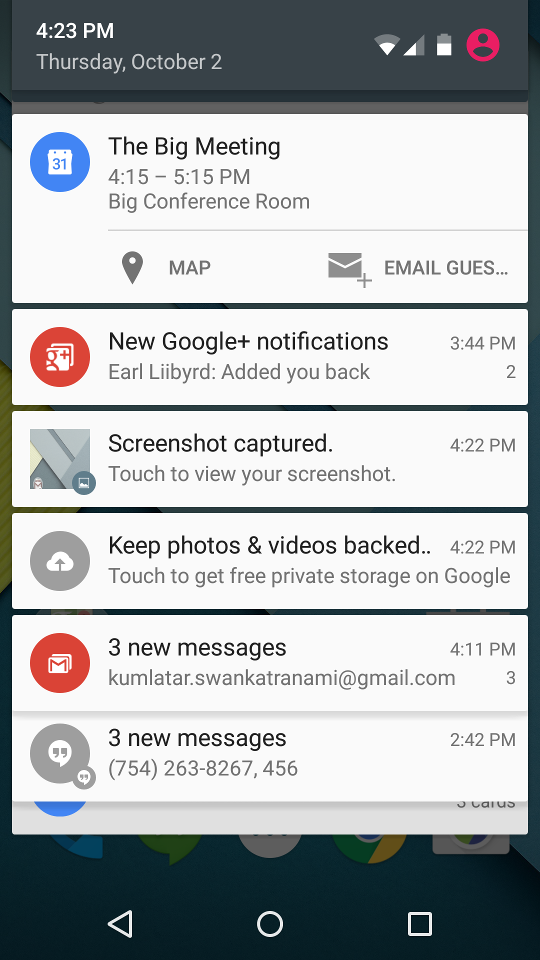
\includegraphics[width=0.3\textwidth]{notification_drawer}
\caption{Exemplo de notificações no Android \cite{notificationDrawer}}
\label{notification-drawer}
\end{figure}

A área de notificação e a gaveta de notificação mostradas na figura \ref{notification-drawer} são áreas controladas pelo
sistema operacional e que o usuário pode visualizar a qualquer momento.

A maioria das notificações possui pelo menos uma ação atrelada a si. Uma ação permite que os usuários direcionem-se
diretamente da notificação para uma tela específica do aplicativo, onde podem visualizar um ou mais eventos ou realizar outros trabalhos.

\section{Trabalhos Relacionados}
\label{trabalhos-relacionados}

\cite{chun2017exploring}
